\documentclass[a4paper,12pt]{article}
\usepackage[a4paper]{geometry}
\usepackage[utf8]{inputenc}            % Use utf8 input encoding
%\usepackage[latin1]{inputenc}         % Use iso 8859-1 encoding
\usepackage[T1]{fontenc}               % T1 fonts (support for accents/diacritics)
\usepackage{lmodern}                   % font with proper T1 support and good glyph quality
\usepackage{listings}                  % for (code) listings
\lstset{language=Java}
\usepackage{amsmath}                   % AMS math typesetting
\usepackage{titlesec}
\usepackage{hyperref}                  % better references for PDF
\usepackage{graphicx}               % for graphics
\usepackage{float}
\usepackage{algorithm}
\usepackage[noend]{algpseudocode}

\titleformat{\section}{\LARGE\bfseries}% hide redundant number
{}{0pt}{}

\graphicspath{{pictures/assignment3/}}
\setlength{\parskip}{2ex plus0.5ex minus0.5ex}
\newcommand{\Maxn}{Max\textsuperscript{n}\ }

\begin{document}
    
    \begin{center}
        \rule{\textwidth}{0.1pt}\\[1cm]
        
        \Large Softwarepraktikum SS 2019\\\bf Assignment 3
    \end{center}
    
    
    \begin{center}
        
        \rule{\textwidth}{0.1pt}\\[0.5cm]
        
        {\Large Group - 6\\[5mm]}
        
        \begin{tabular}{lll}
            
            Roman Vuskov & 376809 & roman.vuskov@rwth-aachen.de \\
            
            Songran Shi & 357791 & songran.shi@rwth-aachen.de \\
            
            Marlene Damm & 379945 & marlene.damm@rwth-aachen.de \\
            
            Marvin Gazibarić & 378154 & marvin.gazibaric@rwth-aachen.de \\
            
        \end{tabular}\\[0.5cm]
        
        \rule{\textwidth}{0.1pt}\\[1cm]
        
    \end{center}
    
    % Uncomment next two lines for table of contents
    \newpage
    %\tableofcontents
    \section{Task 1 \& 2}
    Three different search algorithms were considered for this task: \Maxn search, paranoid search and Best Reply search. In the following sections we will explore the strengths and weaknesses of each algorithm and explain our ultimate decision in favor of Best Reply search. We will also discuss the implementation details of our algorithm as well as alpha-beta pruning.
    
    \subsection{\texorpdfstring{\Maxn Search}{Max\textasciicircum n Search}}
    The most straightforward extension of the standard 2-player Minimax algorithm to multi-player\footnote{Multi-player refers to >2 players} games is the \Maxn algorithm: Instead of assigning each node a single (scalar) value, the valuation of a game state is now represented by a vector with one component for each player. A layer in the game tree still corresponds to a particular player's turn, but he only pays attention to his component of the value vectors when making a move decision.
    
    \begin{figure}[H]
        \centering
        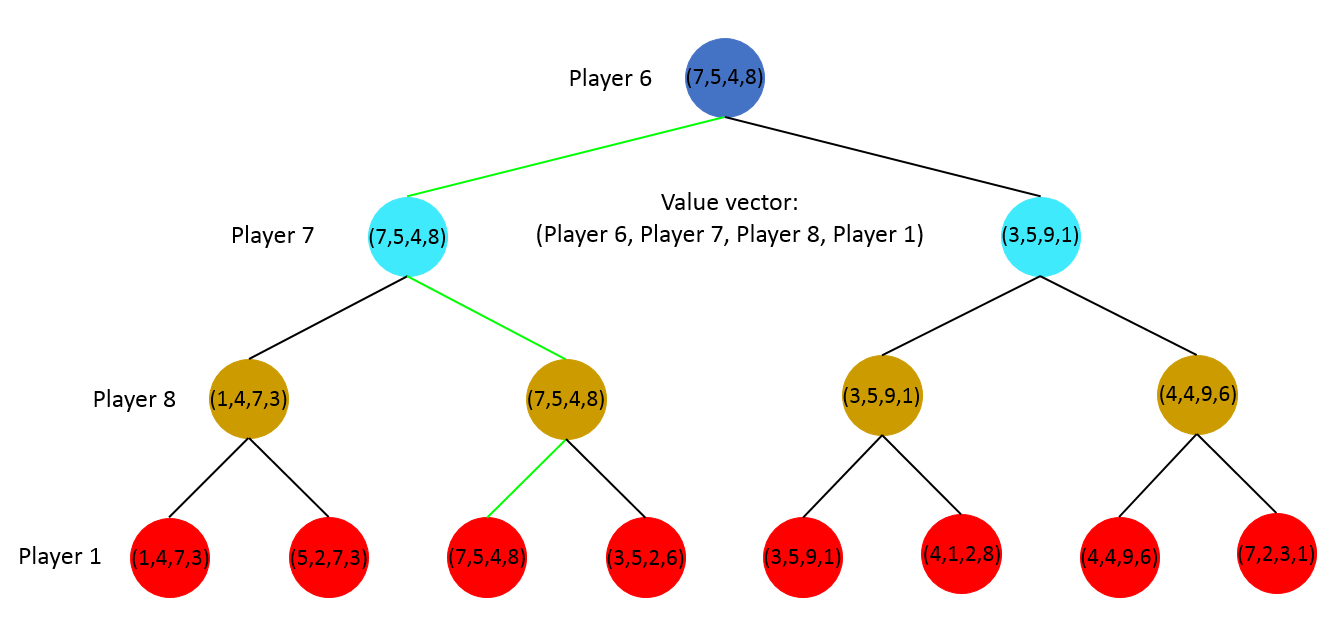
\includegraphics[width=\textwidth,keepaspectratio]{pictures/assignment3/MaxnTree.png}
        \caption{A 4-player \Maxn game tree}
    \end{figure}
    
    The obvious advantage of \Maxn is that it accurately represents the true interest of each player - winning the game - and thus mimics real player behavior the closest. This is an essential property for any game tree search algorithm since looking ahead and gaining a more accurate picture of the future board state evolution is the reason we're utilizing tree searches in the first place. If the results diverge too strongly, we might as well not bother.
    
    However, there is a fatal flaw to this algorithm: It has been mathematically proven \cite{multiplayer-alpha-beta} that there exists no pruning scheme for \Maxn comparable in computational efficiency with alpha-beta pruning in the two-player case, where the branching factor is reduced to $\sqrt{b}$ ($b$ being the branching factor without pruning) in the best case and $b^{3/4}$ realistically. Alternative pruning schemes for \Maxn such as Hypermax \cite{n-person-minimax} only yield a branching factor of $b^{(N-1)/N}$ (where $N$ is the total player count) even in the best case. In the 8-player case, this amounts to an improvement by a factor of only $b^{d/8}$ in search time (where $d$ is the search depth).
    
    \subsection{Paranoid Search}
    An alternative to \Maxn for multi-player games is paranoid search: Here we simply assume the worst case possible where every other player is teaming up against us, each choosing the move that harms our position the most. This assumption allows us to -- just like in the 2-player case -- assign each board state a single value, namely the valuation from our point of view. The game tree then consists of one Max-layer followed by $N-1$ Min-layers:
    
    \begin{figure}[H]
        \centering
        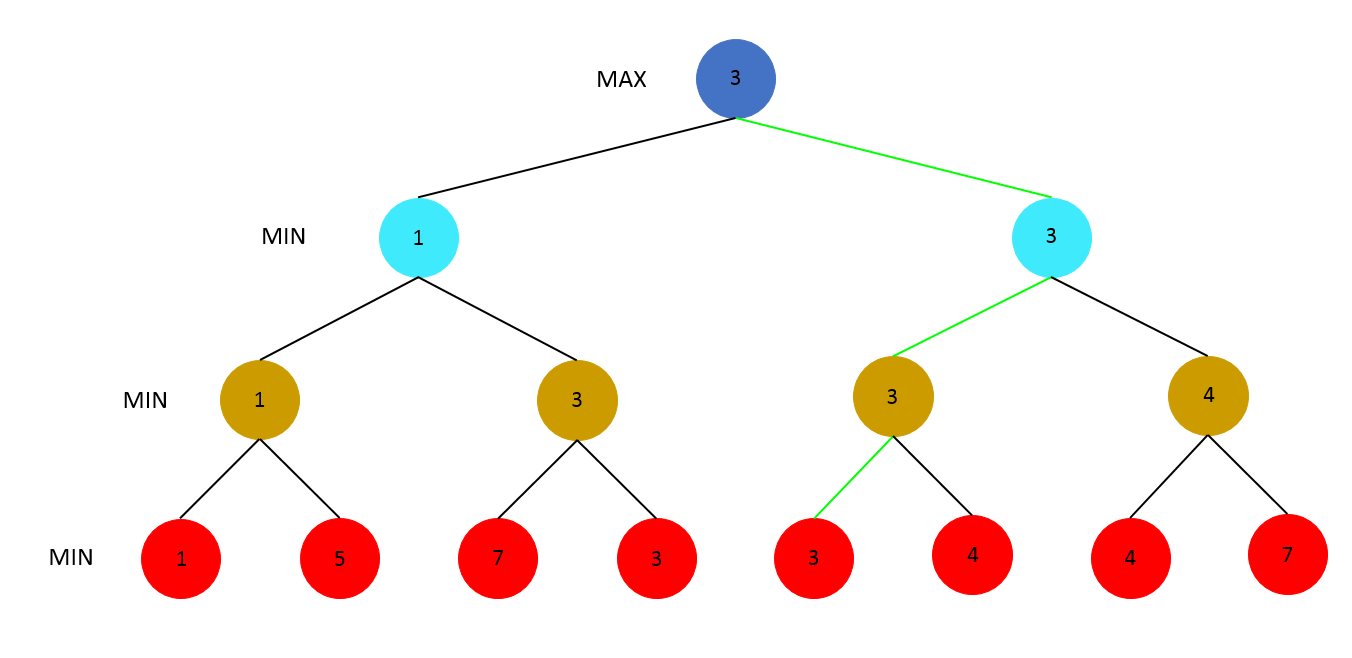
\includegraphics[width=\textwidth,keepaspectratio]{pictures/assignment3/ParanoidSearchTree.png}
        \caption{A paranoid search game tree. The situation is the same as in Figure 1}
    \end{figure}
    
    Since the evaluation of board states return single scalar values again, alpha-beta pruning becomes applicable here in a similar fashion to standard 2-player Minimax. Surprisingly, paranoid search actually performs quite well against \Maxn in experiments \cite{algorithm-comparison}\cite{best-reply-search} with other games. However, there are several reasons to doubt the applicability of these results to Reversi++:
    \begin{enumerate}
        \item In \cite{algorithm-comparison}, it is apparent that paranoid search's win-rate against \Maxn decreases with growing total player count. This is expected as the paranoid assumption deviates more and more from reality with increasing player count: Harming another player's position increasingly becomes a public good
        \item The score of a game in \cite{best-reply-search} is binary: A game counts as either a win or a loss, and there is no reward for second place. In this case it makes sense for all other players to form an alliance against the player in 1\textsuperscript{st} place, and conversely it makes sense for the player in 1\textsuperscript{st} place to be paranoid. This, however, does not apply to the scoring system in Reversi++
        \item A large part of paranoid search's superiority comes from the extra search depth alpha-beta pruning enables. With game boards as large as 2500 tiles in Reversi++ however, either algorithm can only scratch the surface of the whole game tree
    \end{enumerate}
    
    \subsection{Best Reply Search}
    Best Reply Search \cite{best-reply-search} offers a reasonable middle ground between \Maxn and paranoid search. The game tree for Best Reply Search looks very much like the Minimax tree for 2-players, with alternating Max- and Min-layers where the Max-player represents us and the Min-player represents all other players (i.e. has moves of all other players available to him):
    
    \begin{figure}[H]
        \centering
        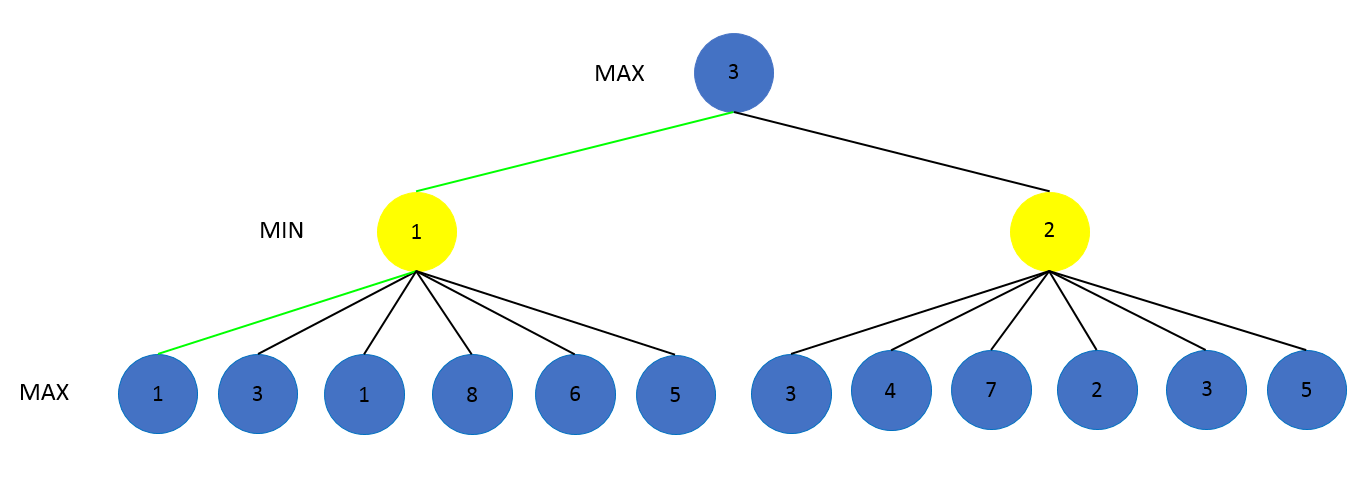
\includegraphics[width=\textwidth,keepaspectratio]{pictures/assignment3/BRSTree.png}
        \caption{A Best Reply Search game tree. MIN has many more nodes than MAX since Min represents all other players}
    \end{figure}
    
    Like paranoid search, the value at each node is a simple scalar, and alpha-beta pruning is even more straightforward here. BRS also makes the paranoid assumption, but not as strongly as paranoid search since the Min-player will only have 50\% of the turns instead of $\frac{N-1}{N}$. Additionally, it has the advantage of searching through more Max-layers -- the layers most relevant to us -- over both \Maxn and paranoid search. This is especially justified in the early stages of the game where usually players' starting positions are divided into pairs, and the pairs are far apart from each other. This way, considering moves of any player other than ourselves and the closest opponent is a waste of computational resources which BRS avoids.
    
    However, it should be noted that BRS mostly produces board states that cannot exist in reality: the BRS game tree is \emph{not} a representation of possible future states. In experiments in \cite{best-reply-search}, though, BRS produced good results against both \Maxn and paranoid search nonetheless, which was the ultimate reason we settled on this algorithm. It would still be worth to conduct tests in Reversi++ with all three algorithms to determine empirically which is best suited for this particular game.
    
    \subsection{Beam Search}
    Even with alpha-beta pruning, the branching factor can still turn out to be too much to handle with the given search depth and time limit. Additionally, alpha-beta pruning requires reasonable ordering of child nodes to provide any significant speedup. To account for both, we introduced beam search into our algorithm: for each node in the tree (except for leave nodes) the AI first finds all child nodes and evaluates the board state of these child nodes directly (essentially a one-step search), then orders the best $w$ of them in a list for the subsequent recursive call. $w$ then is our beam width, or the effective branching factor, and the ordered list of child nodes is the ``beam'' we're searching through. This way, we can control the branching factor of our game tree at any stage of the game:
    
    \begin{figure}[H]
        \centering
        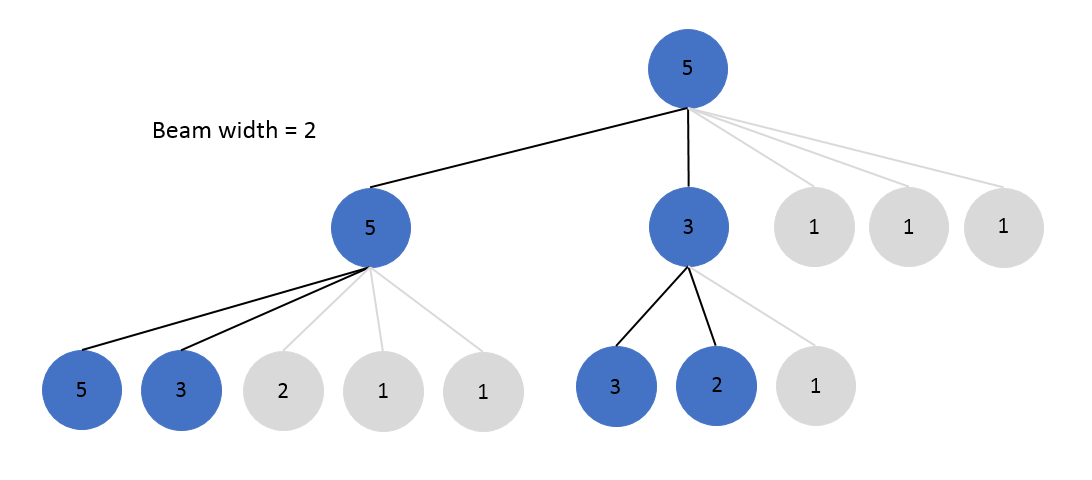
\includegraphics[width=\textwidth,keepaspectratio]{pictures/assignment3/BeamSearch.png}
        \caption{A beam search tree with beam width 2}
    \end{figure}
    
    This is however a greedy strategy since we might be discarding quite a few possible moves at each node on relatively little information. If this turns out to be a bad idea that affects the output quality too much, we can still effectively turn off beam search by setting beam width to infinity while retaining move ordering for alpha-beta pruning to be efficient.
    
    \subsection{Implementation}
    Our implementation of Best Reply Search consists only of one class: the BRSNode class. It contains two constructors and 6 methods:
    \begin{itemize}
        \item \texttt{public BRSNode} \quad public constructor for the root node; used only by external calls
        \item \texttt{private BRSNode} \quad private constructor for internal nodes; only used by (recursive) internal calls
        \item \texttt{getBestMove} \quad simply returns the best move from the node that has already been evaluated; only used on the root node to return the final result
        \item \texttt{evaluateNode} \quad recursive method and center point of the class; first computes search beam (using \texttt{computeBeam}); then constructs for beam entries child nodes and calls \texttt{evaluateNode} in them; finally updates its own value to the maximum or minimum (depending on whether it's a Max- or Min-Node) of its children values and returns its own value
        \item \texttt{computeBeam} \quad computes the beam by fetching all legal moves (by using \texttt{getMaxMoves} or \texttt{getMinMoves}) and ordering the best $w$ of them in a list; then returns the ordered list
        \item \texttt{getMaxMoves} \quad fetches legal moves the Max-player (us) can make; prioritizes regular moves over override moves (it's a good heuristic to save override moves for last)
        \item \texttt{getMinMoves} \quad fetches all other players' legal moves and merges them into one set (these are moves the Min-player can make by definition of BRS); prioritizes regular moves over override moves
        \item \texttt{evaluateCurrentState} \quad evaluates the board state of the node according to heuristics; used to order child nodes and to evaluate leave nodes
    \end{itemize}
    
    \begin{algorithm}[H]
        \caption{Node Evaluation}
        \begin{algorithmic}
            \Function{EvaluateNode}{$ $}
            \Statex
            \State beam[move] $\gets$ \Call{ComputeBeam}{$ $}
            \Statex
            \If{beam is empty}
            \State \textbf{return} value of current state
            \Statex
            \ElsIf{current layer == search depth}
            \State \textbf{return} value of current state
            \Statex
            \ElsIf{this node is Max node}
            \For{\textbf{each} move in beam}
            \State construct child node(current layer + 1, Min node)
            \State \Call{EvaluateNode}{child node}
            \If{child node value > node value}
            \State node value = child node value
            \EndIf
            \EndFor
            \Statex
            \ElsIf{this node is Min node}
            \For{\textbf{each} move in beam}
            \State construct child node(current layer + 1, Max node)
            \State \Call{EvaluateNode}{child node}
            \If{child node value < node value}
            \State node value = child node value
            \EndIf
            \EndFor
            \EndIf
            \EndFunction
        \end{algorithmic}
    \end{algorithm}
    
    To initialize BRS, one needs to construct the root node with parameters \texttt{depth} (search depth), \texttt{branching} (branching factor) and \texttt{prune} (alpha-beta pruning on/off), then evaluate the root node and finally get the best move of the root node. With current heuristics in place our BRS algorithm can search through $\approx 1000$ nodes per second, pending future updates. It is only used for the first phase of the game as moves in the Bombing Phase are mostly independent of each other and the branching factor is very large, making a direct move evaluation more practical than any sort of tree search.
    
    \subsection{Alpha-beta pruning}
    Alpha-beta pruning can be seamlessly integrated into BRS. We initialize $\alpha$ and $\beta$ as $-\infty$ and $+\infty$ respectively, and pass down these two parameters each time a child node is constructed. When a node is going through the beam and updating its own value, $\alpha$ or $\beta$ (depending on whether it's a Max- or Min-Node) is updated as well and compared with each other. If $\beta \leq \alpha$, the loop gets broken and the rest of the beam discarded, as per the alpha-beta pruning algorithm.
    
    \begin{algorithm}[H]
        \caption{Alpha beta Node Evaluation}
        \begin{algorithmic}
            \Function{EvaluateNode}{$ $}
            \Statex
            \State beam[move] $\gets$ \Call{ComputeBeam}{$ $}
            \Statex
            \If{beam is empty}
            \State \textbf{return} value of current state
            \Statex
            \ElsIf{current layer == search depth}
            \State \textbf{return} value of current state
            \Statex
            \ElsIf{this node is Max node}
            \For{\textbf{each} move in beam}
            \State construct child node(current layer + 1, Min node, $\alpha$, $\beta$)
            \State \Call{EvaluateNode}{child node}
            \If{child node value > node value}
            \State node value = child node value
            \State $\alpha$ = child node value
            \If{$\alpha \geq \beta$}
            \State break
            \EndIf
            \EndIf
            \EndFor
            \Statex
            \ElsIf{this node is Min node}
            \For{\textbf{each} move in beam}
            \State construct child node(current layer + 1, Max node, $\alpha$, $\beta$)
            \State \Call{EvaluateNode}{child node}
            \If{child node value < node value}
            \State node value = child node value
            \State $\beta$ = child node value
            \If{$\alpha \geq \beta$}
            \State break
            \EndIf
            \EndIf
            \EndFor
            \EndIf
            \EndFunction
        \end{algorithmic}
    \end{algorithm}
    
    \section{Task 3}
    
    First we compared our AI playing the same map against the same opponents in the same position with and without pruning enabled at depth limit 3. Because pruning does not change the decision outcome the resulting games where the same and easy to compare. 
    \begin{figure}[h!]
        \centering
        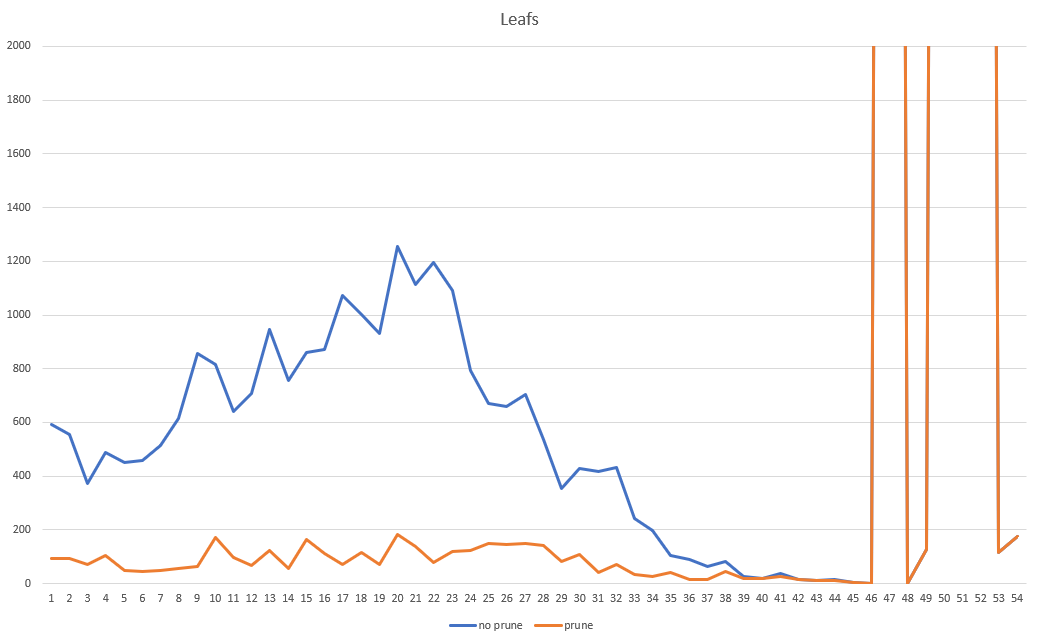
\includegraphics[width = 14cm]{leafs.png}
        \caption{blue without pruning, orange with pruning}
        \label{fig:leafs}
    \end{figure}
    Figure \ref{fig:leafs} shows that alpha-beta pruning can lower the amount of leaf nodes and thereby computational work by an substantial amount. This is possible to such a degree in our case because we already use move sorting for beam search (the actual beam search is turned off in this experiment). The big spikes after Move 48 belong to the ``every player places his override stones phase'' (the blue curve is obstructed by the orange) and have the exact number of leafs in pruning and no pruning mode suggesting that our method of pruning somehow fails in this phase. This has to be further examined. The amount of states statistic looks basically like the amount of leafs statistic which is unsurprising (more states $\to$ more leaves) so we don't further discuss it here. What however is interesting is that the times per state shown in Figure \ref{fig:tps} are higher with pruning and significantly higher in the ``every player places his override stones phase''.
    \begin{figure}[h!]
        \centering
        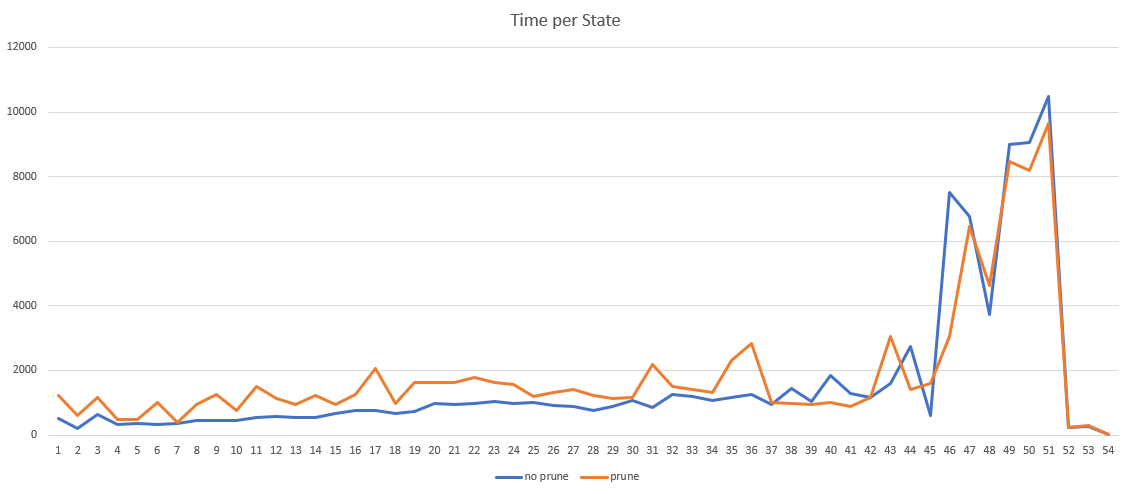
\includegraphics[width = 14cm]{tps.png}
        \caption{blue without pruning, orange with pruning}
        \label{fig:tps}
    \end{figure}
    \begin{figure}[h!]
        \centering
        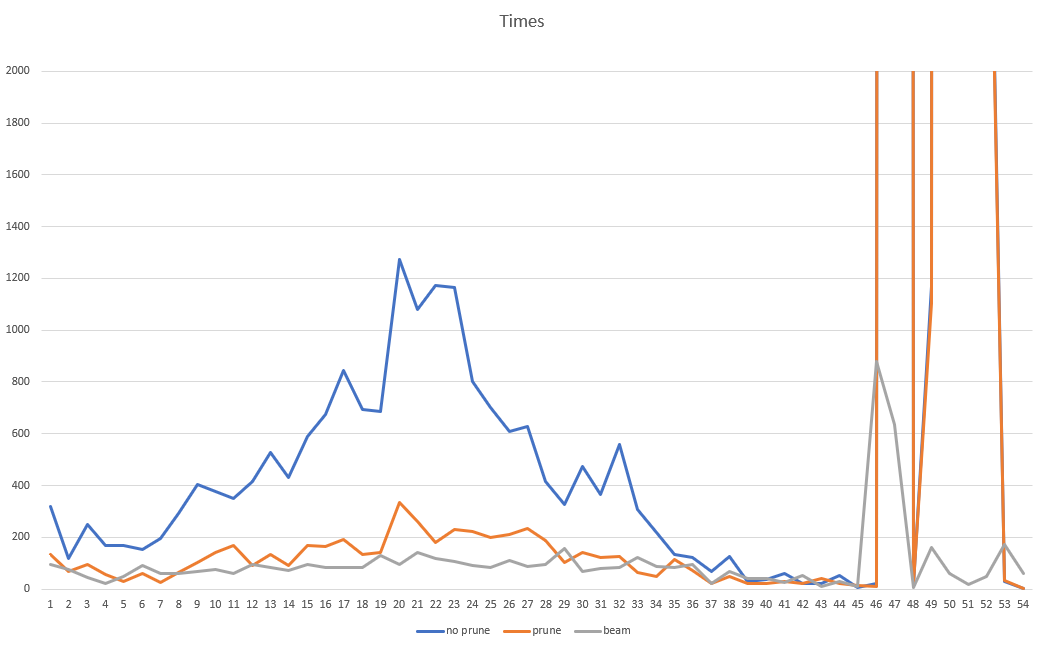
\includegraphics[width = 14cm]{times.png}
        \caption{blue without pruning, orange with pruning, gray beam}
        \label{fig:time}
    \end{figure}
    Figure \ref{fig:time} shows that even though times per state are higher with pruning the AI is able to chose moves faster because there are less states. It also shows how much faster beam search combined with pruning can be. Because beam search introduces a maximum branching factor it can also handle the extreme branching of the ``every player places his override stones phase''.
    
    This of course is not a big sample size but previous research from various people shows that alpha-beta pruning should be used when doing minMax, especially if you are able to do good (and fast) move sorting.     
    \begin{thebibliography}{4}
        \bibitem{multiplayer-alpha-beta} R. E. Korf, “Multiplayer Alpha-Beta Pruning”, Artificial Intelligence, vol. 48, no. 1, pp. 99-111, 1991. 
        
        \bibitem{n-person-minimax} Mikael Fridenfalk, “N-Person Minimax and Alpha-Beta Pruning”, NICOGRAPH International 2014, pp. 43-52 
        
        \bibitem{algorithm-comparison} Nathan Sturtevant, “A Comparison of Algorithms for Multi-player Games”, Computers and Games Third International Conference, CG 2002, pp. 108-122
        
        \bibitem{best-reply-search} Maarten P.D. Schadd and Mark H.M. Winands, “Best-Reply Search for Multi-Player Games”
    \end{thebibliography}
    
\end{document}

